\begin{center}
    \textbf{\Huge{Relatório - \emph{Model Serving}: Práticas e Soluções existentes}}
\end{center}

\section{Introdução}

O propósito deste documento é apresentar uma visão abrangente das práticas atuais e das soluções tecnológicas existentes para model serving, isto é, o processo de disponibilização de modelos de aprendizado de máquina em ambientes de produção com requisitos rigorosos de disponibilidade, desempenho e escalabilidade.

O estudo é conduzido no contexto de ambientes de simulação construtiva, nos quais soluções de model serving precisam se integrar diretamente ao loop de execução da simulação. Em particular, considera-se o domínio de defesa, como simulações de combate aéreo além do alcance visual (Beyond Visual Range – BVR), caracterizadas por execução computacional em alta frequência, com taxas de atualização (ticks) elevadas e restrições severas de latência e previsibilidade temporal.

Nesse cenário, decisões de inferência atrasadas ou inconsistentes podem comprometer a coerência do estado simulado, tornando insuficientes abordagens tradicionais de servimento de modelos concebidas para aplicações assíncronas ou orientadas a requisições independentes. Ao final deste relatório, são discutidas as possibilidades, limitações e adaptações necessárias para a utilização de servidores de modelos no contexto de simulações construtivas de alta fidelidade.

\subsection{Referências}

\begin{itemize}
    \item ROMERO, Francisco et al. {INFaaS}: Automated model-less inference serving. In: 2021 USENIX Annual Technical Conference (USENIX ATC 21). 2021. p. 397-411.
    \item ZHANG, Huaizheng et al. Inferbench: Understanding deep learning inference serving with an automatic benchmarking system. arXiv preprint arXiv:2011.02327, 2020.
    \item GORANTLA, Varun Kumar Chowdary. Microservices Architecture for Scalable Real-Time Data Processing at the Edge. International Journal of Emerging Trends in Computer Science and Information Technology, v. 5, n. 2, p. 53-62, 2024.
    \item SINGH, Jaskirat et al. On the impact of black-box deployment strategies for edge ai on latency and model performance. arXiv preprint arXiv:2403.17154, 2024.
    \item ZHAO, Zhixin et al. SLOpt: Serving real-time inference pipeline with strict latency constraint. IEEE Transactions on Computers, 2025.
    \item LIU, Bote. Study and benchmarking of Artificial Intelligence (AI) model serving systems on edge computation units and cloud environments. 2019.
    \item OLSTON, Christopher et al. Tensorflow-serving: Flexible, high-performance ml serving. arXiv preprint arXiv:1712.06139, 2017.
    \item PIAO, Dongming. The impact of batching on TensorFlow serving performance. In: 2nd International Conference on Mechatronic Automation and Electrical Engineering (ICMAEE 2024). IET, 2024. p. 255-263.
    \item FACONTI, Davide. BehaviorTree.CPP: Integration with ROS2. Disponível em: \url{https://www.behaviortree.dev/docs/ros2_integration/} . Acesso em: 29 jan. 2026
\end{itemize}

\section{Fundamentos de \emph{Model Serving} em Sistemas Modernos}
\subsection{Do Treinamento à Inferência: Mudança de Requisitos}
A transição do treinamento de modelos de aprendizado de máquina para sua execução em produção representa uma mudança fundamental de requisitos e pressupostos. Enquanto o treinamento é tipicamente realizado em ambientes controlados, com cargas previsíveis, execução offline e foco quase exclusivo na maximização da acurácia média, a inferência em produção ocorre sob condições radicalmente distintas, caracterizadas por requisições online, padrões de carga dinâmicos e restrições rígidas de latência e disponibilidade.

Segundo Olston et al., ao descrever o desenvolvimento do TensorFlow Serving, soluções inicialmente simples para servir modelos rapidamente evoluem para sistemas complexos à medida que novos requisitos surgem, como versionamento de modelos, suporte a múltiplas versões simultâneas, rollback seguro e experimentação controlada (A/B testing). Esses requisitos não possuem equivalentes diretos na fase de treinamento e demandam preocupações típicas de sistemas distribuídos, como isolamento de recursos, concorrência e tolerância a falhas.

Essa ruptura conceitual é aprofundada por Romero et al., que argumentam que a inferência não deve ser tratada como a execução estática de um modelo previamente escolhido, mas como um processo dinâmico no qual diferentes variantes de modelos podem ser selecionadas por requisição, de acordo com objetivos de latência, custo e acurácia. Nesse contexto, o desenvolvedor deixa de especificar diretamente “qual modelo servir” e passa a declarar requisitos de serviço, delegando ao sistema a tomada de decisões operacionais.

\begin{table}[htbp]
  \centering
  \caption{Aplicações consultando um mesmo modelo de reconhecimento facial com prioridades diversas (adaptado de Romero, 2021).}
  \label{tab:metrics}

  \begin{tabular}{@{}lccc@{}}
    \toprule
    & \textbf{Acurácia} & \textbf{Latência} & \textbf{Custo} \\ \midrule
    Mídia Social     & Alta   & Média & Baixa   \\
    Guia Visual      & Alta   & Baixa & Alta  \\
    Detecção de Intruso & Baixa & Baixa & Baixa   \\
    \bottomrule
  \end{tabular}
\end{table}

\begin{figure}[htbp]
  \centering
  \begin{verbatim}
register_model("ResNet50", "ResNet50.pt", valSet, detectFaceApp)
register_model("MobileNet", "MobileNet.pt", valSet, detectFaceApp)
# O desenvolvedor registrou 2 modelos para o detectFaceApp;
# INFaaS gera variantes a partir desses dois modelos registrados
inference_query(input.jpg, detectFaceApp, 200ms, 70%)
# O desenvolvedor enviou uma consulta com "input.jpg" como entrada
# e requisitos especificados; INFaaS então seleciona uma variante
# automaticamente para atender à latência de 200ms e precisão >70%
  \end{verbatim}
  \vspace{-1.0cm}
  \caption{Registrando modelos e submetendo consultas ao INFaaS (adaptado de Romero, 2021).}
  \label{fig:infass-code}
\end{figure}

Adicionalmente, Zhang et al. observam que essa mudança de requisitos não é apenas operacional, mas também metodológica. A ausência de práticas sistemáticas de avaliação da inferência antes da implantação em produção contribui para um descompasso entre o desempenho esperado durante o desenvolvimento e o comportamento real do sistema em operação. Assim, a inferência emerge como uma fase distinta do ciclo de vida de sistemas de aprendizado de máquina, com necessidades próprias de validação, monitoramento e ajuste contínuo.

\subsection{Métricas-Chave: Latência, Throughput, Custo e Confiabilidade}
Em ambientes de produção, métricas tradicionais utilizadas durante o desenvolvimento de modelos são insuficientes para caracterizar adequadamente o desempenho de sistemas de inferência. Conforme destacado por Olston et al., métricas como throughput médio ou tempo médio de resposta não capturam fenômenos críticos observados em sistemas reais, especialmente aqueles relacionados à latência de cauda, que afeta diretamente a experiência do usuário e o cumprimento de acordos de nível de serviço.

Zhang et al. reforçam essa visão ao demonstrar que o desempenho da inferência depende da interação entre múltiplas dimensões, incluindo o modelo, o hardware, o software de servimento e o padrão de workload. Dessa forma, métricas devem ser analisadas de maneira conjunta, considerando não apenas eficiência média, mas também previsibilidade, estabilidade sob carga e consumo de recursos.

O trabalho de Piao evidencia de forma empírica os conflitos entre essas métricas ao analisar o impacto do batching em sistemas de servimento. Embora o aumento do tamanho de batch possa melhorar significativamente o throughput e a eficiência do uso de aceleradores, esse ganho frequentemente ocorre à custa de maior latência, especialmente na cauda da distribuição. Esses efeitos tornam explícito que otimizações locais podem gerar degradações globais no comportamento do sistema.

Além disso, custo operacional emerge como uma métrica de primeira ordem. Segundo Romero et al., decisões subótimas de configuração e escalonamento podem levar a desperdício significativo de recursos computacionais, especialmente em ambientes de nuvem heterogêneos. Assim, latência, throughput, custo e confiabilidade devem ser tratados como objetivos interdependentes, exigindo abordagens de otimização multiobjetivo no projeto de sistemas de servimento.

\begin{table}[htbp]
  \centering
  \caption{Latência, taxa de saturação e custo normalizado (com base nos preços da AWS) para três variantes do ResNet50 (adaptado de Romero, 2021).}
  \label{tab:variantes_resnet}

  \begin{tabular}{@{}lccc@{}}
    \toprule
    & \textbf{Lat. (ms)} & \textbf{Req/s} & \textbf{Custo ($\$$/s)} \\ \midrule
    Variante A (4 CPUs, TensorFlow)          & 200 & 5   & 1   \\
    Variante B (1 núcleo Inferentia, Neuron)  & 20  & 100 & 3   \\
    Variante C (1 GPU V100, TensorRT)        & 15  & 800 & 16  \\ 
    \bottomrule
  \end{tabular}
\end{table}

\subsection{Desafios Sistêmicos em Ambientes de Produção}
Sistemas de servimento de modelos enfrentam desafios que só se manifestam plenamente em ambientes de produção, sob cargas reais e concorrência entre múltiplos serviços. Olston et al. destacam problemas como interferência entre modelos durante operações de carregamento e descarregamento, gerenciamento inadequado de memória e efeitos adversos de operações internas aparentemente secundárias, que podem introduzir picos de latência inesperados.

O estudo de Piao complementa essa análise ao mostrar que mecanismos amplamente utilizados, como batching, introduzem acoplamentos implícitos entre requisições independentes. Em cenários de carga variável, esse acoplamento pode amplificar atrasos, reduzir previsibilidade e dificultar o ajuste fino do sistema para atender requisitos de tempo real.

Esses problemas tornam-se ainda mais pronunciados em sistemas mais complexos, como pipelines de inferência compostos por múltiplos modelos. Zhao et al. demonstram que, em tais cenários, efeitos como head-of-line blocking, cold starts e amplificação de defeitos podem se propagar ao longo do pipeline, resultando em violações sistemáticas de SLOs, mesmo quando cada componente individual aparenta estar corretamente dimensionado.

A Figura~\ref{fig:zhao-blocking}, reproduzida de Zhao et al., ilustra de forma clara como esses efeitos emergem em pipelines de inferência compostos. Mesmo quando a carga de entrada e a capacidade de processamento de cada modelo aparentam estar adequadamente balanceadas individualmente (Fig.~\ref{fig:zhao-blocking}(a)), o sistema apresenta uma taxa elevada de violação de SLO no nível end-to-end (Fig.~\ref{fig:zhao-blocking}(b)).

\begin{figure}[htbp]
    \centering
    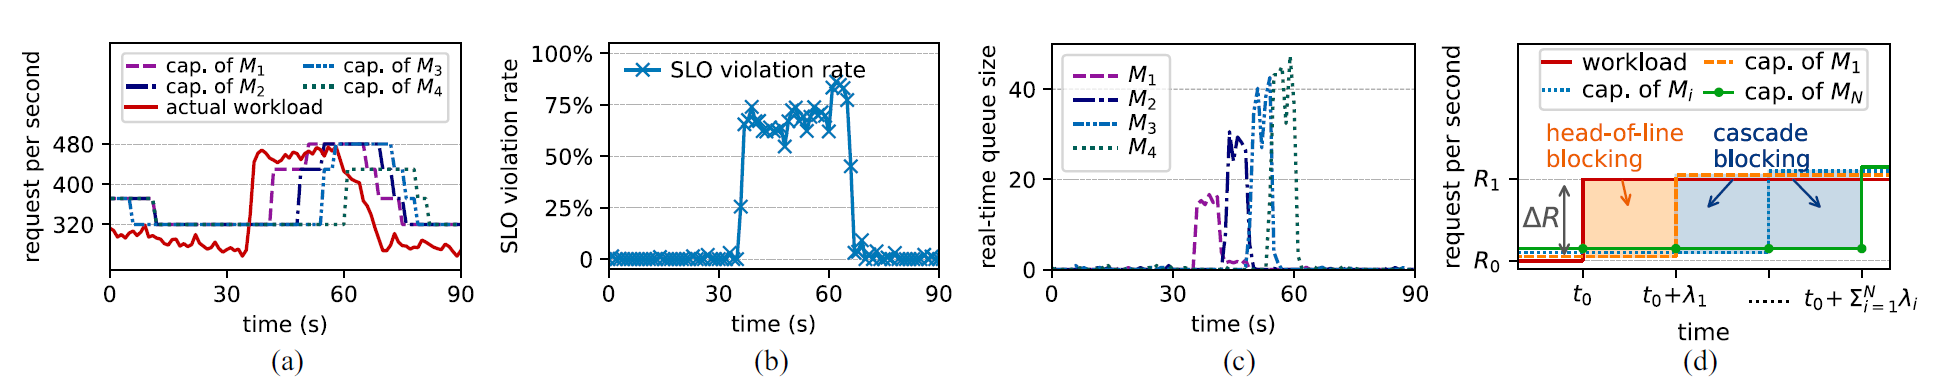
\includegraphics[width=\textwidth]{./content/img/zhao_pipeline_blocking.png}
    \caption{Ilustração dos efeitos de \emph{head-of-line blocking} e \emph{cascade blocking} em pipelines de inferência (reproduzida de Zhao et al, 2025).}
    \label{fig:zhao-blocking}
\end{figure}

A análise das filas em tempo real (Fig.~\ref{fig:zhao-blocking}(c)) revela que atrasos introduzidos nos estágios iniciais do pipeline se propagam para os modelos subsequentes, levando ao acúmulo progressivo de requisições. Esse comportamento caracteriza o fenômeno de cascade blocking, no qual pequenas variações locais de carga ou latência são amplificadas ao longo do pipeline.

Conforme esquematizado na Fig.~\ref{fig:zhao-blocking}(d), esse efeito se combina com head-of-line blocking, fazendo com que requisições atrasadas bloqueiem o processamento de requisições subsequentes, mesmo quando recursos computacionais estão disponíveis. Como consequência, estratégias de escalonamento que tratam modelos de forma isolada tornam-se incapazes de evitar violações sistemáticas de SLOs, evidenciando a necessidade de abordagens conscientes da estrutura e da dinâmica global do pipeline.

Em conjunto, esses desafios evidenciam que o servimento de modelos não pode ser tratado como um problema isolado de execução eficiente de código, mas como um problema sistêmico que envolve arquitetura, escalonamento, automação e avaliação contínua. Essa constatação fundamenta o desenvolvimento de sistemas mais avançados, que incorporam consciência explícita de SLOs, adaptação dinâmica e mecanismos robustos de mitigação de latência.

\section{Arquiteturas de Servimento}
\subsection{Servimento Centralizado em Nuvem}
As primeiras soluções de servimento de modelos em produção foram predominantemente centralizadas e orientadas à nuvem, explorando a disponibilidade de recursos computacionais abundantes e a facilidade de gerenciamento oferecida por data centers centralizados. A arquitetura modular adotada pelo TensorFlow Serving, ilustrada na Fig.~\ref{fig:olston-tfserving}, reflete esse modelo centralizado. Segundo Olston et al., o TensorFlow Serving foi concebido inicialmente nesse contexto, assumindo a nuvem como ambiente primário para hospedar múltiplos modelos e versões, com forte ênfase em desempenho, disponibilidade e facilidade de integração com pipelines de treinamento.

\begin{figure}[htbp]
    \centering
    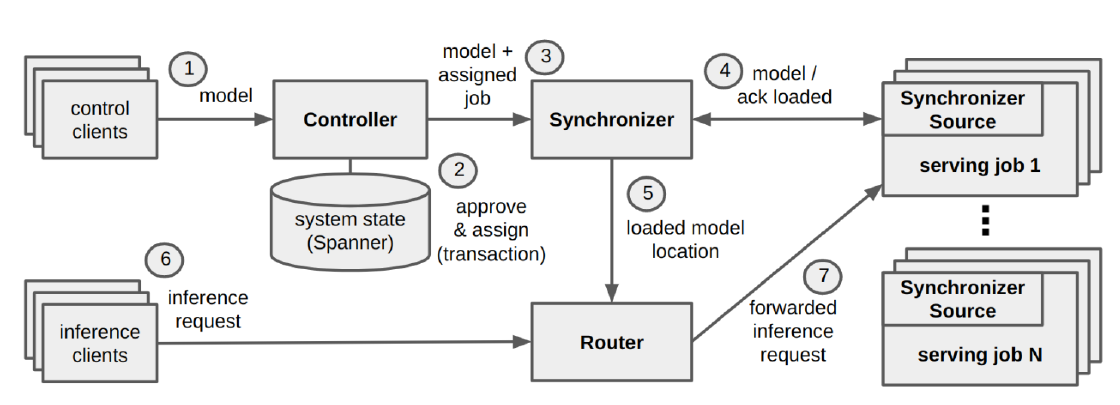
\includegraphics[width=0.8\textwidth]{./content/img/olston_tfserving_architecture.png}
    \caption{Arquitetura do TFS$^2$ - Tensorflow Serving (reproduzida de Olston et al., 2017).}
    \label{fig:olston-tfserving}
\end{figure}

Nesse modelo centralizado, a inferência é tratada como um serviço acessado remotamente, geralmente por meio de chamadas RPC, permitindo consolidar cargas e maximizar a utilização de aceleradores especializados, como GPUs e TPUs. Romero et al. expandem essa visão ao explorar ambientes de nuvem heterogêneos, nos quais diferentes tipos de hardware coexistem e podem ser explorados dinamicamente para atender requisitos distintos de latência, custo e acurácia.

Entretanto, esses trabalhos também evidenciam limitações inerentes à centralização. A dependência da rede, a variabilidade de latência e os custos associados à transmissão de grandes volumes de dados tornam o modelo puramente centralizado menos adequado para aplicações sensíveis a tempo real ou com restrições de privacidade. Essas limitações motivam a exploração de arquiteturas mais distribuídas, especialmente em cenários de Edge AI.

\subsection{Servimento Distribuído e Edge AI}
Arquiteturas distribuídas de servimento emergem como resposta direta às limitações do modelo centralizado, deslocando parte ou a totalidade da inferência para mais próximo das fontes de dados. Segundo Liu, o servimento de modelos em dispositivos de borda reduz significativamente a latência de rede e o consumo de largura de banda, mas introduz novos desafios relacionados à limitação de recursos computacionais e à heterogeneidade do ambiente.

Singh et al. aprofundam essa análise ao tratar o servimento como um continuum entre dispositivos móveis, nós de edge e a nuvem. O estudo demonstra que diferentes estratégias de implantação, incluindo quantização, particionamento de modelos e execução híbrida, produzem trade-offs distintos entre latência, custo e acurácia, dependendo das características do modelo, da rede e do hardware disponível. Como ilustrado na Fig.~\ref{fig:singh-edge}, essas estratégias não são excludentes, mas organizam-se em um continuum.

\begin{figure}[htbp]
    \centering
    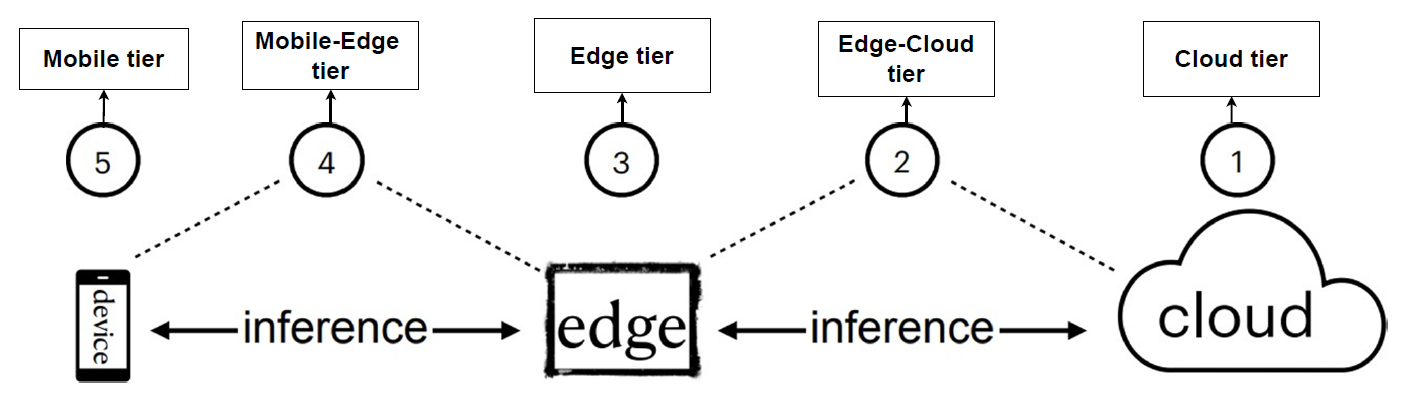
\includegraphics[width=\textwidth]{./content/img/singh_mobile_edge_cloud.png}
    \caption{Visão gráfica das estratégias de implantação de IA na borda em camadas únicas (Mobile, Edge, Cloud) e múltiplas (Mobile‑Edge, Edge‑Cloud) (reproduzida de Singh et al, 2024).}
    \label{fig:singh-edge}
\end{figure}

Esses resultados indicam que arquiteturas distribuídas não substituem completamente o modelo centralizado, mas o complementam. Em muitos cenários, a solução mais eficaz envolve a combinação coordenada de múltiplos níveis de execução, exigindo mecanismos sofisticados de orquestração e decisão arquitetural.

\subsection{Arquiteturas Baseadas em Microserviços}
A adoção de microserviços como estilo arquitetural tem impacto direto no projeto de sistemas de servimento de modelos, especialmente em ambientes distribuídos e de edge computing. Gorantla argumenta que a decomposição de sistemas monolíticos em serviços independentes aumenta a modularidade, a escalabilidade e a tolerância a falhas, características desejáveis em aplicações de inferência em tempo real.

Nesse contexto, cada componente do pipeline de inferência pode ser tratado como um serviço independente, permitindo escalonamento diferenciado, isolamento de falhas e atualização incremental. Embora o trabalho de Gorantla não seja focado exclusivamente em aprendizado de máquina, seus princípios arquiteturais se alinham com práticas observadas em sistemas de servimento modernos.

\begin{table}[htbp]
  \centering
  \caption{Comparação de Escalabilidade entre Arquiteturas de Microsserviços e Monolíticas (adaptado de Gorantla, 2024)}
  \label{tab:escalabilidade}
  \begin{tabular}{@{}lcc@{}}
    \toprule
    & \textbf{Microsserviços (Edge)} & \textbf{Monolítico (Cloud Central)} \\ \midrule
    Eficiência de Escala           & 92\%                         & 68\%                           \\
    Custo por 1M de Requisições   & \$14,20                      & \$18,90                        \\
    Tempo de Recuperação (Failover)& 2.1\,s                       & 8.7\,s                         \\
    Resposta do Auto‑Scaling       & 12–15\,s                     & 45–60\,s                       \\ 
    \bottomrule
  \end{tabular}
\end{table}

O TensorFlow Serving também reflete essa abordagem ao adotar uma arquitetura modular interna, na qual componentes responsáveis por carregamento de modelos, roteamento de requisições e execução de inferência são desacoplados. Essa modularidade facilita a adaptação do sistema a diferentes cenários de implantação e prepara o terreno para integrações mais complexas, como pipelines compostos e ambientes multi-tenant.

\subsection{Pipelines de Inferência e Composição de Modelos}
À medida que aplicações de aprendizado de máquina se tornam mais complexas, cresce a necessidade de arquiteturas capazes de suportar pipelines de inferência compostos por múltiplos modelos encadeados. Zhao et al. destacam que esse paradigma, conhecido como model cascading, permite reutilizar modelos pré-treinados para construir soluções complexas sem a necessidade de treinar redes monolíticas de grande porte.

No entanto, a composição de modelos introduz desafios arquiteturais significativos. Cada estágio do pipeline impõe dependências temporais e de recursos que afetam o comportamento global do sistema. Zhao et al. demonstram que arquiteturas tradicionais, que tratam cada modelo de forma isolada, são incapazes de garantir o cumprimento de SLOs estritos em pipelines encadeados.

Romero et al. abordam esse problema de forma complementar ao propor sistemas que selecionam dinamicamente variantes de modelos e recursos subjacentes, considerando o impacto global da decisão sobre o desempenho do serviço. Embora o INFaaS não trate explicitamente pipelines como entidades de primeira classe, sua abordagem de seleção dinâmica fornece os mecanismos necessários para lidar com composições complexas em ambientes heterogêneos.

Em conjunto, esses trabalhos evidenciam que arquiteturas modernas de servimento precisam ir além do modelo “um modelo, um serviço”, incorporando suporte explícito à composição, coordenação e otimização global de pipelines de inferência.

\section{Gerenciamento de Recursos e Escalonamento}
\subsection{Escalonamento Horizontal e Vertical}
O escalonamento de sistemas de servimento de modelos envolve decisões tanto no eixo horizontal, por meio da replicação de serviços, quanto no eixo vertical, via ajuste da quantidade e do tipo de recursos atribuídos a cada instância. Segundo Olston et al., abordagens iniciais de escalonamento horizontal são eficazes para absorver aumentos de carga, mas rapidamente se tornam ineficientes quando aplicadas de forma indiscriminada, levando a desperdício de memória e degradação de latência durante operações como carregamento de modelos.

Romero et al. avançam essa discussão ao propor um modelo híbrido de escalonamento, no qual a replicação de instâncias é combinada com a seleção dinâmica de variantes de modelos dentro de uma mesma máquina. Essa abordagem permite explorar melhor a heterogeneidade de hardware disponível na nuvem, reduzindo custos e aumentando a flexibilidade do sistema frente a variações de carga.

Em ambientes de edge computing, Liu observa que o escalonamento vertical é frequentemente limitado por restrições físicas do hardware, tornando a replicação inviável ou custosa. Nesses cenários, decisões de escalonamento precisam considerar cuidadosamente o balanceamento entre consumo de recursos locais e dependência da nuvem, reforçando que estratégias eficazes são altamente dependentes do contexto de implantação.
\subsection{Batching, Paralelismo e Efeitos Colaterais}
Batching é uma das técnicas mais utilizadas para aumentar a eficiência de sistemas de inferência, especialmente quando aceleradores como GPUs e TPUs estão envolvidos. Conforme discutido por Olston et al., o batching assíncrono permite consolidar requisições e melhorar a utilização do hardware, mas introduz novos desafios relacionados à latência e à previsibilidade do sistema.

O estudo de Piao fornece uma análise detalhada desses trade-offs ao demonstrar que aumentos no tamanho do batch tendem a melhorar o throughput, porém frequentemente à custa de maior latência, especialmente na cauda da distribuição. O autor mostra que esses efeitos são não lineares e altamente sensíveis à configuração, tornando difícil a escolha de parâmetros ótimos estáticos.

Além disso, o paralelismo excessivo pode levar à contenção de recursos, como threads e memória, resultando em degradação global do desempenho. Esses efeitos colaterais evidenciam que batching não é apenas uma otimização local, mas uma política de escalonamento que deve ser cuidadosamente integrada ao restante do sistema.
\subsection{Gerenciamento de Cauda de Latência (Tail Latency)}
A latência de cauda representa um dos principais desafios no servimento de modelos em produção, pois pequenos atrasos em uma fração das requisições podem comprometer a experiência do usuário ou violar acordos de nível de serviço. Olston et al. destacam que operações internas do sistema, como carregamento e descarregamento de modelos ou liberação de grandes blocos de memória, podem introduzir picos de latência que afetam requisições concorrentes.

Zhang et al. reforçam a importância de medir e analisar explicitamente a latência de cauda ao avaliar sistemas de servimento. Segundo os autores, métricas médias mascaram comportamentos patológicos que só se manifestam sob determinadas configurações ou padrões de carga, dificultando a identificação de gargalos reais.

Zhao et al. abordam o problema de forma mais direta ao tratar a latência de cauda como um objetivo explícito de otimização. Em sistemas de pipelines de inferência, os autores demonstram que a latência de pior caso pode ser amplificada à medida que requisições atravessam múltiplos estágios, exigindo mecanismos específicos de controle e coordenação para manter o cumprimento de SLOs.
\subsection{Cold Start, Head-of-Line Blocking e Amplificação de Atraso}
Fenômenos como cold start e head-of-line blocking são particularmente problemáticos em sistemas de inferência sujeitos a cargas dinâmicas. Segundo Olston et al., o carregamento inicial de modelos ou a ativação de novas réplicas pode introduzir atrasos significativos, afetando requisições que, em princípio, não deveriam ser impactadas por essas operações.

Zhao et al. formalizam esses problemas no contexto de pipelines de inferência, mostrando como atrasos em estágios iniciais podem bloquear o processamento de requisições subsequentes, mesmo quando recursos estão disponíveis em estágios posteriores. Esse efeito, conhecido como head-of-line blocking, contribui para a amplificação de atrasos ao longo do pipeline, tornando o comportamento do sistema difícil de prever.

Além disso, decisões incorretas de provisionamento sob cargas bursty podem levar à acumulação de requisições em filas, agravando ainda mais a latência de cauda. Esses fenômenos evidenciam a necessidade de estratégias de escalonamento conscientes do estado global do sistema, capazes de antecipar variações de carga e mitigar efeitos de amplificação antes que eles se tornem críticos.

\section{Automação e Otimização do Processo de Inferência}
\subsection{Seleção Dinâmica de Modelos e Variantes}
A seleção dinâmica de modelos e suas variantes surge como resposta direta à complexidade crescente dos ambientes de servimento e à diversidade de requisitos das aplicações. Segundo Romero et al., a prática tradicional de selecionar uma única variante de modelo e escalá-la horizontalmente é inadequada em cenários nos quais diferentes requisições apresentam restrições distintas de latência, custo e acurácia.

O INFaaS propõe um paradigma no qual o desenvolvedor especifica apenas objetivos de alto nível, como limites máximos de latência ou requisitos mínimos de acurácia, enquanto o sistema seleciona dinamicamente, para cada requisição, a combinação mais adequada de modelo, variante e hardware subjacente. Essa abordagem explora um espaço amplo de variantes geradas a partir de modelos previamente treinados, incorporando otimizações como quantização, ajustes de batch e uso de aceleradores especializados.

\begin{figure}[htbp]
    \centering
    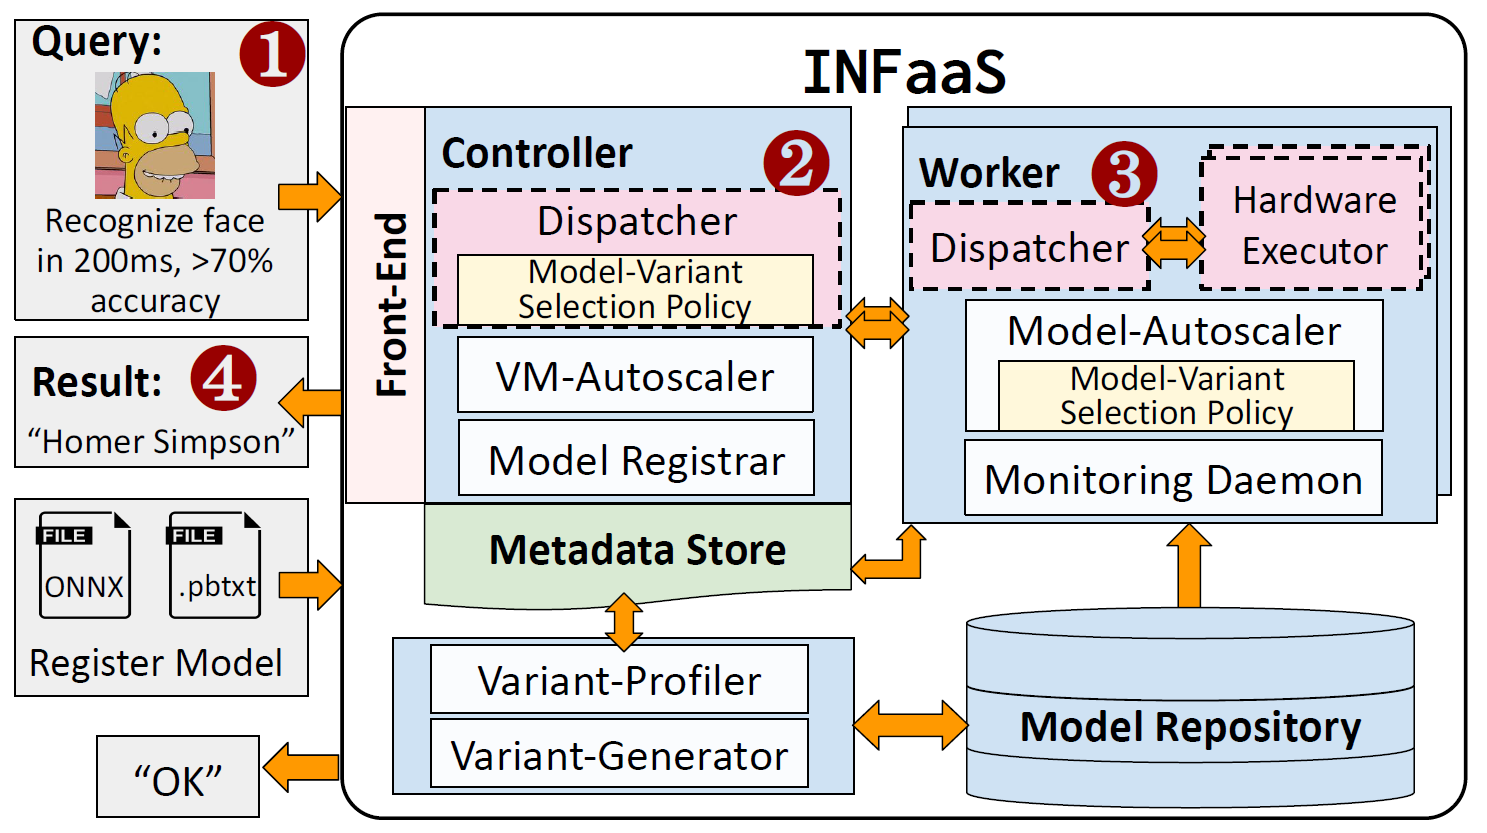
\includegraphics[width=0.8\textwidth]{./content/img/romero_infaas_architecture.png}
    \caption{Arquitetura do INFaaS. Os módulos em caixas com borda tracejada estão no caminho crítico de atendimento de consultas. Todos os demais módulos não afetam a latência de serviço. Os círculos numerados correspondem ao ciclo de vida típico das consultas (reproduzida de Romero, 2021).}
    \label{fig:romero-infaas}
\end{figure}

Essa seleção por requisição permite responder de forma mais eficiente a variações de carga e heterogeneidade de hardware, reduzindo custos e melhorando o cumprimento de objetivos de serviço. Ao mesmo tempo, desloca a complexidade da configuração manual para mecanismos automatizados de decisão, marcando uma mudança significativa no papel do desenvolvedor no ciclo de vida do servimento.
\subsection{Otimizações Transparente ao Desenvolvedor}
A automação do processo de inferência também se manifesta na incorporação de otimizações que são deliberadamente ocultadas do desenvolvedor final. Olston et al. destacam que o TensorFlow Serving codifica diversas boas práticas diretamente na infraestrutura, como estratégias de carregamento seguro de modelos, isolamento entre versões e políticas de batching assíncrono, reduzindo a necessidade de decisões explícitas por parte dos usuários do sistema.

Romero et al. avançam essa ideia ao remover completamente a necessidade de escolha explícita de variantes de modelos. No INFaaS, otimizações como seleção de hardware, ajuste de paralelismo e escolha de configurações de execução são realizadas automaticamente, com base em modelos de desempenho e observação contínua do comportamento do sistema.

Essa transparência traz benefícios claros em termos de produtividade e redução de erros de configuração, mas também introduz novos desafios. A opacidade das decisões automatizadas pode dificultar a depuração de problemas e a compreensão do comportamento do sistema, exigindo ferramentas adequadas de monitoramento e explicabilidade para manter a confiança do operador.
\subsection{Servimento Sensível a SLOs e Restrições de Latência}
A incorporação explícita de objetivos de nível de serviço (SLOs) representa um passo adicional na automação de sistemas de servimento. Zhao et al. argumentam que abordagens reativas, baseadas apenas em métricas observadas, são insuficientes para garantir o cumprimento de restrições rigorosas de latência, especialmente em pipelines de inferência compostos por múltiplos modelos encadeados.

O SLOpt introduz um sistema de servimento projetado desde o início para tratar SLOs como entidades de primeira classe. Por meio de estimativas antecipadas de workload, provisionamento proativo de recursos e políticas adaptativas de execução, o sistema busca minimizar a latência de cauda, em especial métricas como P99, mesmo sob cargas bursty e padrões de acesso dinâmicos.

\begin{figure}[htbp]
    \centering
    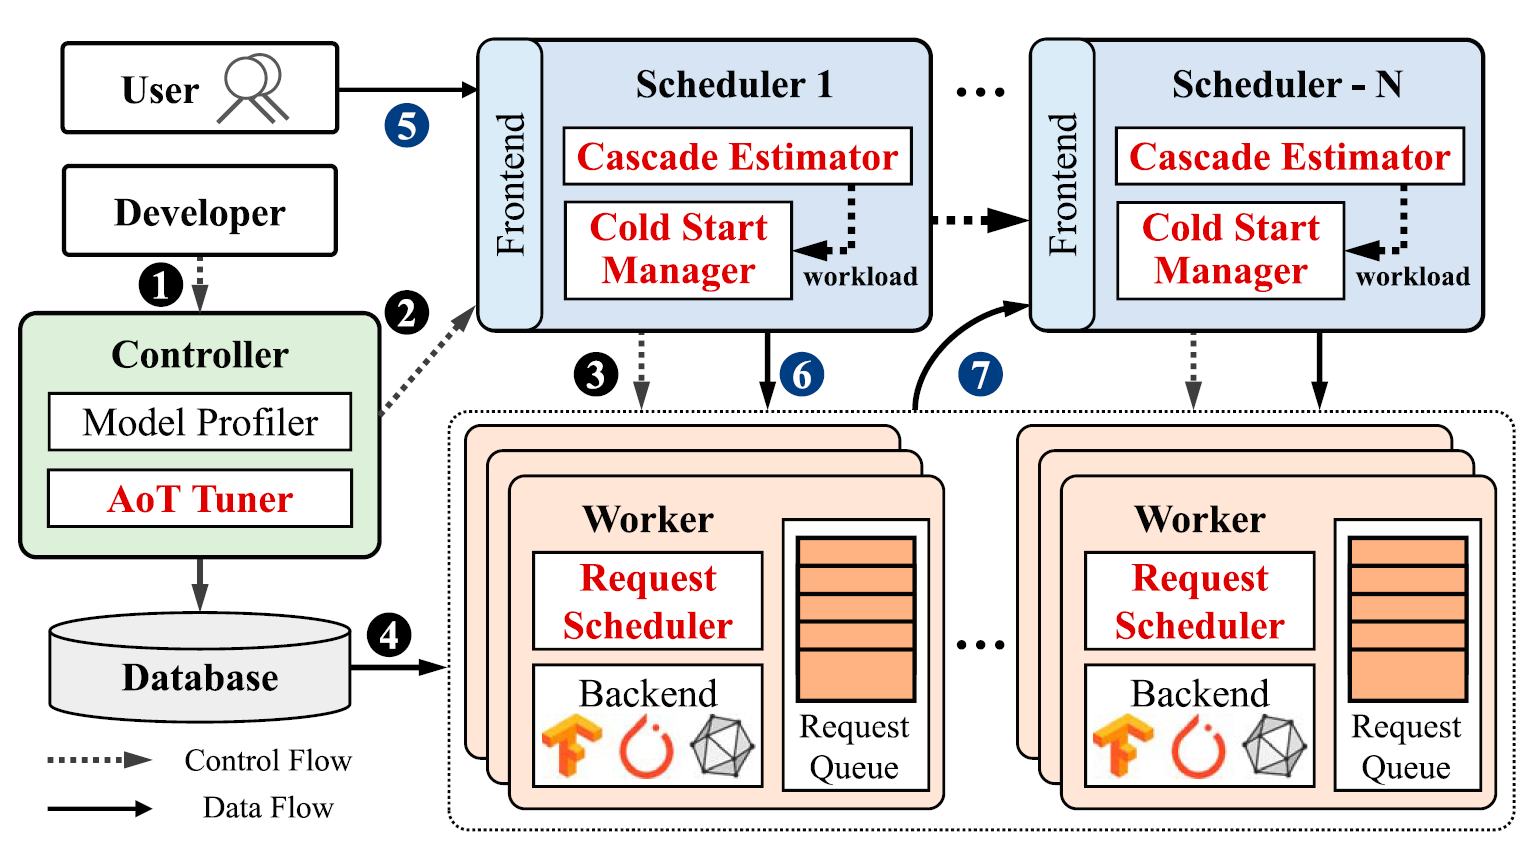
\includegraphics[width=0.8\textwidth]{./content/img/zhao_slopt_overview.png}
    \caption{Overview do SLOpt (reproduzida de Zhao et. al., 2025).}
    \label{fig:zhao-slopt}
\end{figure}

Embora Romero et al. não tratem explicitamente pipelines encadeados, o INFaaS compartilha a filosofia de otimização orientada a objetivos, ao selecionar dinamicamente variantes de modelos e recursos para atender restrições impostas por diferentes aplicações. Em conjunto, esses trabalhos indicam uma tendência clara em direção a sistemas de servimento que não apenas executam inferência de forma eficiente, mas que também raciocinam continuamente sobre como cumprir objetivos de serviço em ambientes complexos e heterogêneos.

\section{Benchmarking e Avaliação de Sistemas de Servimento}
\subsection{Benchmarks Sintéticos vs Cargas Realistas}
A avaliação de sistemas de servimento de modelos tradicionalmente recorre a benchmarks sintéticos, que oferecem controle e reprodutibilidade, mas frequentemente falham em representar o comportamento observado em produção. Zhang et al. argumentam que muitos estudos avaliam inferência utilizando workloads simplificados, modelos únicos e configurações fixas, o que limita a validade externa dos resultados obtidos.

O InferBench foi projetado explicitamente para lidar com essa limitação ao permitir a geração automática de workloads variados, incluindo diferentes tamanhos de batch, arquiteturas de modelos, formatos de entrada e padrões de requisição. Segundo os autores, essa flexibilidade possibilita explorar sistematicamente o espaço de configuração do servimento, aproximando a avaliação de cenários reais sem abrir mão da reprodutibilidade.

Em contrapartida, Liu destaca que cargas realistas frequentemente envolvem restrições adicionais, como limitações severas de hardware em dispositivos de edge e variações significativas na latência de rede. Esses fatores são difíceis de capturar em benchmarks puramente sintéticos, reforçando a necessidade de combinar avaliações controladas com experimentação em ambientes representativos do mundo real.

Assim, a literatura indica que benchmarks sintéticos e cargas realistas não devem ser vistos como abordagens concorrentes, mas como instrumentos complementares para compreender o comportamento de sistemas de servimento sob diferentes perspectivas.
\subsection{Impacto de Hardware, Software e Configuração}
O desempenho de sistemas de inferência é fortemente influenciado pela interação entre hardware, software de servimento e parâmetros de configuração. Zhang et al. demonstram que variações aparentemente pequenas, como o tipo de acelerador utilizado ou o tamanho do batch, podem resultar em diferenças substanciais de latência, throughput e custo operacional.

O InferBench explicita essa dependência ao organizar a avaliação em múltiplas camadas, incluindo hardware, infraestrutura de servimento e pipeline de execução. Essa abordagem permite identificar gargalos específicos e compreender como decisões em uma camada afetam o comportamento global do sistema.

Piao reforça essa visão ao analisar o impacto de configurações de batching em TensorFlow Serving. Seus resultados mostram que o mesmo modelo pode apresentar comportamentos drasticamente distintos dependendo do hardware subjacente e das políticas de escalonamento adotadas, tornando inviável a extrapolação direta de resultados entre ambientes diferentes.

De forma complementar, Singh et al. evidenciam que, em cenários de Edge AI, o impacto do hardware e da configuração é amplificado pela variabilidade da rede e pelas restrições dos dispositivos. Estratégias eficazes em ambientes de nuvem podem se tornar inviáveis ou contraproducentes quando aplicadas em contextos móveis ou de borda.
\subsection{Ferramentas e Metodologias de Avaliação Automatizada}
A complexidade do espaço de configuração de sistemas de servimento torna a avaliação manual impraticável em larga escala. Nesse contexto, Zhang et al. propõem o InferBench como uma ferramenta de benchmarking automatizada, capaz de gerar workloads, executar experimentos e coletar métricas de forma sistemática e reprodutível.

O sistema incorpora mecanismos para evitar interferência entre experimentos concorrentes e fornece ferramentas de análise que auxiliam na interpretação dos resultados. Segundo os autores, essa automação reduz significativamente o esforço necessário para avaliar novas configurações e facilita a comparação justa entre diferentes arquiteturas e estratégias de servimento.

Embora Liu e Singh et al. não proponham ferramentas de benchmarking automatizadas no mesmo nível, seus trabalhos reforçam a importância de metodologias experimentais cuidadosas, que considerem múltiplos fatores simultaneamente e evitem conclusões baseadas em cenários excessivamente simplificados.

Em conjunto, esses estudos indicam que a avaliação de sistemas de servimento deve ser tratada como um processo contínuo e automatizado, integrado ao ciclo de vida do sistema, em vez de uma etapa pontual realizada apenas durante o desenvolvimento.

\section{Trade-offs em Ambientes Heterogêneos}
\subsection{Cloud vs Edge vs Mobile}
A escolha entre executar inferência na nuvem, na borda ou diretamente em dispositivos móveis envolve trade-offs estruturais que vão além de simples considerações de desempenho. Segundo Liu, a inferência em nuvem se beneficia de recursos computacionais abundantes e aceleradores especializados, mas sofre com latência de rede e maior dependência de conectividade, o que pode ser inadequado para aplicações sensíveis a tempo real.

Em contraste, a execução na borda reduz a latência de comunicação e o consumo de largura de banda, aproximando o processamento da fonte de dados. No entanto, Liu observa que dispositivos de edge frequentemente apresentam limitações severas de CPU, memória e capacidade de escalonamento, o que restringe o tipo de modelo e a carga que podem ser suportados de forma sustentável.

Singh et al. ampliam essa análise ao tratar cloud, edge e mobile como partes de um continuum arquitetural. Seus experimentos demonstram que a melhor estratégia de implantação depende fortemente das características do modelo, do tamanho dos dados de entrada e das condições da rede. Em alguns cenários, a nuvem oferece melhor desempenho global, enquanto em outros a execução parcial ou total na borda ou no dispositivo móvel se mostra mais eficaz.

Esses resultados indicam que não existe uma estratégia universal de implantação. Em vez disso, sistemas modernos de servimento precisam ser capazes de adaptar dinamicamente a localização da inferência às condições do ambiente e aos requisitos da aplicação.
\subsection{Precisão vs Latência vs Custo}
Outro eixo fundamental de trade-off em ambientes heterogêneos envolve a relação entre precisão do modelo, latência de inferência e custo operacional. Romero et al. destacam que diferentes aplicações valorizam essas métricas de forma distinta, e que a escolha de uma única configuração fixa frequentemente leva a soluções subótimas.

O INFaaS aborda esse problema ao permitir que o sistema selecione dinamicamente variantes de modelos que atendam aos requisitos de cada requisição. Essa abordagem evidencia que pequenas reduções de precisão podem resultar em ganhos significativos de latência ou economia de custos, especialmente quando variantes otimizadas ou hardware especializado são utilizados.

Singh et al. fornecem evidências empíricas desses trade-offs no contexto de Edge AI, mostrando que técnicas como quantização, early exit e particionamento de modelos produzem diferentes compromissos entre precisão e tempo de resposta, dependendo do tier de execução. Em alguns casos, perdas moderadas de acurácia são compensadas por reduções substanciais de latência, enquanto em outros a preservação da precisão exige maior custo computacional ou dependência da nuvem.

Zhao et al. complementam essa discussão ao introduzir restrições explícitas de SLO, mostrando que o custo necessário para manter níveis elevados de precisão e latência previsível pode crescer rapidamente em pipelines complexos. Assim, a otimização em ambientes heterogêneos é inerentemente multiobjetivo e depende de decisões informadas sobre quais métricas priorizar em cada contexto.
\subsection{Impacto da Rede e da Localidade dos Dados}
A rede desempenha um papel central na definição dos trade-offs em ambientes heterogêneos, especialmente quando a inferência é distribuída entre múltiplos tiers. Singh et al. demonstram que a largura de banda e a latência da rede influenciam diretamente a viabilidade de estratégias como particionamento de modelos e execução híbrida entre edge e cloud.

Os resultados mostram que modelos com entradas grandes ou intermediárias volumosas são particularmente sensíveis a limitações de rede, tornando estratégias distribuídas inviáveis em cenários de baixa largura de banda. Em contrapartida, modelos com entradas menores podem ser eficientemente executados na nuvem mesmo sob restrições de conectividade.

Liu reforça essa observação ao destacar que a localidade dos dados afeta não apenas a latência, mas também questões de privacidade e custo de transmissão. A necessidade de enviar grandes volumes de dados para a nuvem pode introduzir riscos adicionais e custos operacionais significativos, especialmente em aplicações contínuas ou de alta frequência.

Esses trabalhos evidenciam que decisões arquiteturais em ambientes heterogêneos não podem ignorar as características da rede. A localidade dos dados e a qualidade da conexão tornam-se fatores determinantes na escolha da estratégia de servimento, exigindo sistemas capazes de adaptar suas decisões às condições dinâmicas do ambiente.

\section{Limitações Atuais e Lacunas de Pesquisa}
\subsection{Generalização de Resultados Experimentais}
Uma limitação recorrente nos trabalhos analisados diz respeito à dificuldade de generalizar resultados experimentais para cenários distintos daqueles avaliados. Zhang et al. reconhecem que, embora o InferBench permita explorar sistematicamente um amplo espaço de configurações, os resultados obtidos ainda dependem fortemente do conjunto de modelos, hardware e padrões de workload considerados nos experimentos.

De forma semelhante, Piao demonstra que conclusões sobre o impacto do batching são altamente sensíveis a parâmetros específicos, como tipo de acelerador, configuração de threads e características do modelo. Assim, configurações consideradas ótimas em um ambiente podem se mostrar inadequadas ou até prejudiciais em outro, limitando a transferência direta de boas práticas entre sistemas.

Em ambientes heterogêneos, essa limitação é ainda mais pronunciada. Liu e Singh et al. mostram que resultados obtidos em contextos específicos de cloud ou edge não se estendem automaticamente a outros cenários, especialmente quando variáveis como largura de banda, capacidade computacional e tamanho dos dados de entrada variam significativamente.

Essas observações indicam que, embora os estudos forneçam resultados interessantes, ainda há uma lacuna na construção de modelos de desempenho verdadeiramente generalizáveis, capazes de orientar decisões de servimento em ambientes diversos sem necessidade de extensa experimentação local.
\subsection{Complexidade Operacional em Escala}
À medida que sistemas de servimento evoluem para incorporar automação, heterogeneidade de hardware e pipelines complexos, a complexidade operacional cresce de forma significativa. Olston et al. já apontavam que sistemas aparentemente simples rapidamente se transformam em infraestruturas difíceis de manter, exigindo cuidados rigorosos com versionamento, isolamento e gerenciamento de recursos.

Romero et al. reconhecem que, embora o INFaaS reduza a carga cognitiva do desenvolvedor ao automatizar decisões de seleção e escalonamento, essa automação introduz novos desafios operacionais. A necessidade de manter catálogos de variantes, modelos de desempenho atualizados e mecanismos confiáveis de monitoramento aumenta a complexidade interna do sistema.

Zhao et al. demonstram que sistemas sensíveis a SLO, como o SLOpt, exigem coordenação sofisticada entre estimativas de workload, provisionamento de recursos e políticas de execução. Em larga escala, pequenos erros de previsão ou atrasos na adaptação podem resultar em violações sistemáticas de SLOs ou em custos excessivos.

Esses trabalhos evidenciam que a escalabilidade não é apenas um problema de desempenho, mas também de operabilidade. Ferramentas de observabilidade, depuração e controle tornam-se essenciais, mas ainda são tratadas de forma secundária na maioria das propostas acadêmicas.
\subsection{Desafios em Ambientes Dinâmicos e Multi-Tenant}
Ambientes dinâmicos e multi-tenant representam um dos maiores desafios ainda abertos no servimento de modelos. Olston et al. observam que a coexistência de múltiplos modelos e versões em um mesmo sistema pode gerar interferência imprevisível, especialmente quando operações de manutenção ou atualização ocorrem simultaneamente à inferência.

Zhang et al. mostram que até mesmo o processo de benchmarking pode sofrer interferência significativa em ambientes compartilhados, dificultando a obtenção de medições confiáveis. Esse problema é amplificado em sistemas multi-tenant, nos quais workloads concorrentes com prioridades distintas disputam os mesmos recursos.

Romero et al. e Zhao et al. abordam parcialmente esses desafios por meio de isolamento lógico e decisões automatizadas, mas ambos reconhecem que lidar com workloads altamente dinâmicos e requisitos conflitantes permanece um problema em aberto. Em particular, garantir justiça, previsibilidade e eficiência simultaneamente em ambientes compartilhados continua sendo uma questão não resolvida.

Além disso, em cenários de edge e mobile, Singh et al. destacam que a variabilidade do ambiente, incluindo mobilidade, flutuações de rede e mudanças no perfil de carga, torna ainda mais difícil manter garantias estáveis de desempenho.

Em conjunto, essas limitações apontam para a necessidade de pesquisas futuras que integrem de forma mais profunda modelagem de incerteza, adaptação contínua e mecanismos robustos de isolamento em sistemas de servimento de modelos.

\subsection{Servimento de Lógicas de Decisão e Modelos Estado-dependentes}

Grande parte da literatura sobre \emph{model serving} concentra-se no servimento de modelos estatísticos, em particular redes neurais profundas, assumindo um paradigma de inferência \emph{stateless} e orientado a requisições independentes. No entanto, em diversos domínios práticos, especialmente em robótica, jogos e simulação construtiva, mecanismos de decisão baseados em lógica estruturada, como \emph{Behavior Trees} (BTs), são amplamente utilizados para controlar agentes autônomos de forma reativa, modular e previsível.

Diferentemente de modelos de aprendizado de máquina tradicionais, \emph{Behavior Trees} são avaliados de forma cíclica, geralmente em sincronia com um \emph{loop} de controle ou com o \emph{tick} da simulação, mantendo dependências temporais explícitas entre avaliações consecutivas. Essa característica introduz um forte acoplamento entre tempo lógico, estado interno e frequência de execução, tornando inadequadas abordagens de servimento baseadas exclusivamente em chamadas remotas assíncronas ou em arquiteturas projetadas prioritariamente para maximizar \emph{throughput}.

Nesse contexto, o servimento de BTs aproxima-se mais de um problema de \emph{orquestração de execução distribuída} do que de inferência tradicional. A introdução de latência variável, \emph{jitter} ou perdas ocasionais de avaliação pode comprometer a coerência do comportamento do agente, mesmo quando a lógica de decisão é determinística. Assim, métricas clássicas de desempenho, como latência média, tornam-se menos relevantes do que garantias de periodicidade, previsibilidade temporal e sincronização rigorosa com o ciclo de controle.

A literatura relacionada ao \emph{Robot Operating System} (ROS) aborda parcialmente esses desafios ao empregar \emph{Behavior Trees} como mecanismo de decisão de alto nível em sistemas robóticos distribuídos. Em particular, a biblioteca BehaviorTree.CPP fornece suporte explícito à integração com ROS2 por meio de \emph{wrappers} para ações e serviços, permitindo a execução reativa e não bloqueante de árvores de comportamento dentro de nós ROS2 (FACONTI, 2026). Ainda assim, essas abordagens assumem predominantemente execução local ou comunicação de baixa latência, explorando de forma limitada mecanismos de escalonamento dinâmico, isolamento de recursos e garantias explícitas de SLOs, como aqueles discutidos em sistemas modernos de \emph{model serving}.

No contexto de simulações construtivas e ambientes de defesa, nos quais lógicas de decisão baseadas em BTs podem coexistir com modelos de aprendizado de máquina em pipelines híbridos, torna-se necessário repensar o próprio conceito de servimento. Em vez de tratar \emph{Behavior Trees} como modelos a serem inferidos sob demanda, é mais apropriado considerá-los como serviços de execução contínua, sensíveis ao \emph{tick} e fortemente acoplados ao tempo lógico da simulação. Essa perspectiva evidencia uma lacuna relevante na literatura atual e abre espaço para arquiteturas híbridas, nas quais inferência estatística e lógica de decisão são servidas de forma coordenada, respeitando restrições temporais, requisitos de previsibilidade e consistência global do sistema.

\section{Considerações Finais}

\subsection{Síntese dos achados}

Este relatório apresentou uma análise sistemática das principais práticas, arquiteturas e soluções existentes para \emph{model serving} em ambientes de produção, evidenciando que o servimento de modelos de aprendizado de máquina constitui um problema eminentemente sistêmico. A literatura analisada demonstra de forma consistente que decisões locais de otimização, como \emph{batching}, paralelismo ou escalonamento reativo, frequentemente introduzem efeitos colaterais que se manifestam na forma de aumento da latência de cauda, interferência entre \emph{workloads} e violações de acordos de nível de serviço. Trabalhos como TensorFlow Serving, InferBench, INFaaS e SLOpt mostram que métricas médias são insuficientes para caracterizar o comportamento real desses sistemas, sendo necessário adotar abordagens que considerem explicitamente variabilidade, previsibilidade temporal e trade-offs entre latência, custo e acurácia. Em conjunto, os estudos indicam uma tendência clara de evolução do \emph{model serving} de soluções estáticas e centradas em infraestrutura para sistemas adaptativos, orientados a objetivos e conscientes de SLOs.

\subsection{Implicações para simulação construtiva}

No contexto de simulações construtivas de alta fidelidade, como aquelas empregadas em cenários de defesa e combate aéreo além do alcance visual (\emph{Beyond Visual Range} -- BVR), os desafios identificados tornam-se particularmente críticos. Diferentemente de aplicações tradicionais orientadas a requisições independentes, simulações construtivas operam em \emph{loops} temporais rígidos, nos quais atrasos ou variações na inferência podem comprometer a coerência global do estado simulado. Os fenômenos de \emph{head-of-line blocking}, \emph{cascade blocking} e amplificação de latência ao longo de pipelines de inferência, discutidos na literatura, indicam que abordagens convencionais de \emph{model serving} não são diretamente aplicáveis a esse domínio sem adaptações substanciais. Nesse cenário, soluções que incorporam consciência explícita de SLOs, coordenação global entre estágios de inferência e seleção dinâmica de modelos e recursos mostram-se mais promissoras, desde que alinhadas às restrições temporais impostas pelo mecanismo de simulação.

\subsection{Limites do estudo e próximos passos}

Embora o relatório tenha coberto um conjunto representativo de trabalhos relevantes, este estudo possui limitações inerentes. A análise baseia-se predominantemente em resultados experimentais reportados na literatura, os quais são fortemente dependentes de configurações específicas de hardware, \emph{workloads} e ambientes de execução, limitando a generalização direta das conclusões. Além disso, poucos trabalhos abordam explicitamente o acoplamento entre \emph{model serving} e mecanismos de simulação com requisitos temporais determinísticos. Como próximos passos, destacam-se a necessidade de experimentação prática em ambientes de simulação construtiva, a avaliação empírica de políticas adaptativas de inferência sob \emph{ticks} rígidos e o desenvolvimento de modelos de desempenho que integrem inferência, escalonamento e tempo lógico da simulação. Esses avanços são fundamentais para viabilizar o uso robusto e previsível de servidores de modelos em cenários de simulação complexos e sensíveis a tempo real.

